\documentclass{standalone}
\usepackage{tikz}

\usetikzlibrary{calc}


\begin{document}

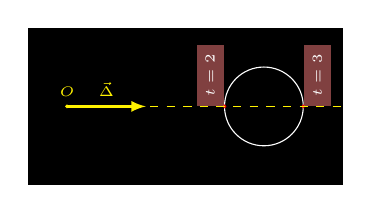
\begin{tikzpicture}
  \path[fill=black] (-2,-1) rectangle (2,1);

  \coordinate (C) at (1,0);
  \coordinate (P1) at ($ (C) + (180:0.5) $);
  \coordinate (P2) at ($ (C) + (0:0.5) $);
  \coordinate (O) at ($ (P1) ! -2 ! (P2) $);

  \draw[white] (C) circle [radius=0.5cm];

  \path[fill=red] (P1) circle [radius=0.025cm] node[fill=red!50,opacity=0.5,text opacity=1,rotate=90,anchor=south west,font=\tiny] {\color{white} $t = 2$};
  \path[fill=red] (P2) circle [radius=0.025cm] node[fill=red!50,opacity=0.5,text opacity=1,rotate=90,anchor=north west,font=\tiny] {\color{white} $t = 3$};

  \draw[dashed,yellow] (O) -- ($ (P1) ! 1.5 ! (P2) $);
  \path[fill=yellow] (O) circle [radius=0.025cm] node[above,font=\tiny,yellow] {$O$};
  \draw[-latex,thick,yellow] (O) -- ($ (O) ! 1cm ! (P1) $) node[midway,above,sloped,font=\tiny] {$\vec\Delta$};
\end{tikzpicture}

\end{document}